\documentclass[12pt,a4paper]{article}
\usepackage[utf8]{inputenc}
\usepackage[english]{babel}

\usepackage{amsmath}
\usepackage{amsfonts}
\usepackage{amssymb}

\usepackage{graphicx}
\usepackage{caption}
\usepackage{subcaption}
\usepackage{lmodern}
\usepackage{tikz}
\usepackage{titlesec}
\usepackage{environ}
\usepackage{xcolor}
\usepackage{fancyhdr}
\usepackage[colorlinks = true, linkcolor = black]{hyperref}
\usepackage{xparse}
\usepackage{enumitem}
\usepackage{comment}
\usepackage{wrapfig}
\usepackage[capitalise]{cleveref}

\usepackage[left=2cm,right=2cm,top=2cm,bottom=2cm]{geometry}
\usepackage{multicol}
\usepackage[indent=0pt]{parskip}

\newcommand{\spaceP}{\vspace*{0.5cm}}
\newcommand{\Span}{\mathrm{Span}\,}
\newcommand{\range}{\mathrm{range}\,}
\newcommand{\ra}{\rightarrow}

%% Redefining sections
\newcommand{\sectionformat}[1]{%
    \begin{tikzpicture}[baseline=(title.base)]
        \node[rectangle, draw] (title) {#1};
    \end{tikzpicture}
    
    \noindent\hrulefill
}

\newif\ifhNotes 

\hNotesfalse

\ifhNotes
	\newcommand{\hideNotes}[1]{%
	\phantom{#1}
	}
	\newcommand{\hideNotesU}[1]{%
	\underline{\hspace{1mm}\phantom{#1}\hspace{1mm}}
	}
\else
	\newcommand{\hideNotes}[1]{#1}
	\newcommand{\hideNotesU}[1]{\textcolor{blue}{#1}}
\fi

% default values copied from titlesec documentation page 23
% parameters of \titleformat command are explained on page 4
\titleformat%
    {\section}% <command> is the sectioning command to be redefined, i. e., \part, \chapter, \section, \subsection, \subsubsection, \paragraph or \subparagraph.
    {\normalfont\large\scshape}% <format>
    {}% <label> the number
    {0em}% <sep> length. horizontal separation between label and title body
    {\centering\sectionformat}% code preceding the title body  (title body is taken as argument)

%% Set counters for sections to none
\setcounter{secnumdepth}{0}

%% Set the footer/headers
\pagestyle{fancy}
\fancyhf{}
\renewcommand{\headrulewidth}{0pt}
\renewcommand{\footrulewidth}{2pt}
\lfoot{P.-O. Paris{\'e}}
\cfoot{MATH 302}
\rfoot{Page \thepage}

%% Defining example environment
\newcounter{example}[section]
\NewEnviron{example}%
	{%
	\noindent\refstepcounter{example}\fcolorbox{gray!40}{gray!40}{\textsc{\textcolor{red}{Example~\theexample.}}}%
	%\fcolorbox{black}{white}%
		{  %\parbox{0.95\textwidth}%
			{
			\BODY
			}%
		}%
	}

% Theorem environment
\NewEnviron{theorem}%
	{%
	\noindent\refstepcounter{example}\fcolorbox{gray!40}{gray!40}{\textsc{\textcolor{blue}{Theorem~\theexample.}}}%
	%\fcolorbox{black}{white}%
		{  %\parbox{0.95\textwidth}%
			{
			\BODY
			}%
		}%
	}

\NewEnviron{notes}%
	{%
	\noindent \fcolorbox{gray!40}{gray!40}{\textsc{\textcolor{blue}{Solution.}}}%
	%\fcolorbox{black}{white}%
		{  %\parbox{0.95\textwidth}%
			{
			\textcolor{blue}{%
			\BODY
			}
			}%
		}%
	}
%%% Ignorer les notes
\excludecomment{notes}

%%%%
\begin{document}
\thispagestyle{empty}

\begin{center}
\vspace*{2.5cm}

{\Huge \textsc{Math 302}}

\vspace*{2cm}

{\LARGE \textsc{Chapter 8}} 

\vspace*{0.75cm}

\noindent\textsc{Section 8.3: Unit Step Function}

\vspace*{0.75cm}

\tableofcontents

\vfill

\noindent \textsc{Created by: Pierre-Olivier Paris{\'e}} \\
\textsc{Fall 2022}
\end{center}

\newpage

\section{Piecewise Continuous Functions}
A piecewise continuous function $f$ is
	\begin{itemize}
	\item a function defined on a finite number of intervals $[t_0, t_1]$, $[t_1, t_2]$, $\ldots$, $[t_{n-1} , t_n]$;
	\item such that it is continuous on each interval $(t_0, t_1)$, $(t_1 , t_2)$, $\ldots$, $(t_{n-1}, t_n)$.
	\end{itemize}
	
	\vspace*{16pt}
	
	\begin{figure}[ht]
	\centering
		\begin{subfigure}[b]{0.45\textwidth}
			\centering
			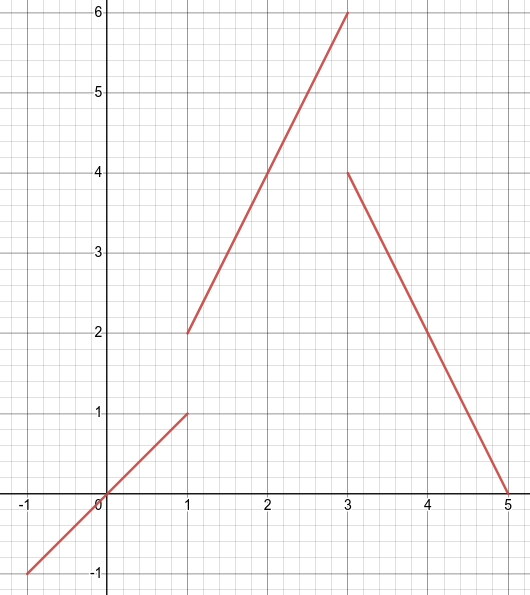
\includegraphics[scale=0.35]{PieceCont1.png}
			\caption{A function $f(x)$}
		\end{subfigure}
		\vspace*{12pt}
		
		\begin{subfigure}[b]{1\textwidth}
			\centering
			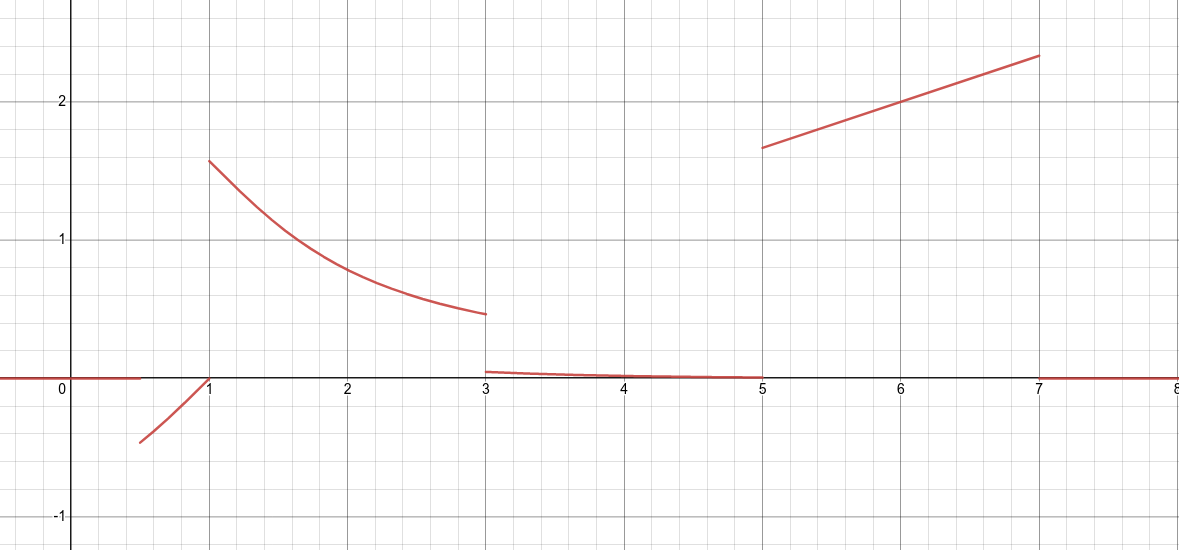
\includegraphics[scale=0.25]{PieceCont4.png}
			\caption{A function $k(x)$}
		\end{subfigure}
		\vspace*{12pt}
		
		\begin{subfigure}[b]{0.45\textwidth}
			\centering
			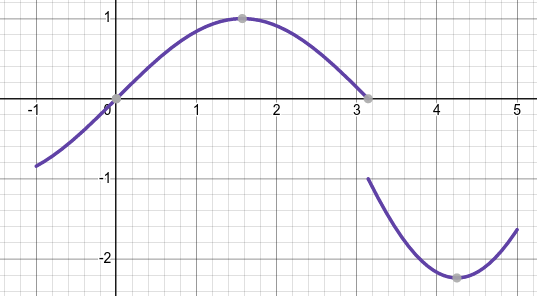
\includegraphics[scale=0.4]{PieceCont2.png}
			\caption{A function $g(x)$}
		\end{subfigure}
		\hfill
		\begin{subfigure}[b]{0.45\textwidth}
			\centering
			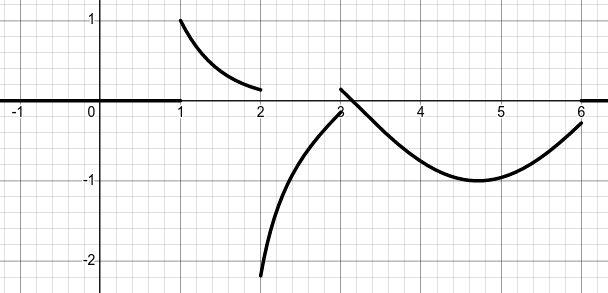
\includegraphics[scale=0.35]{PieceCont3.png}
			\caption{A function $h(x)$}
		\end{subfigure}
	\end{figure}
	
	\newpage
	
	\begin{example}\label{Exa:PieceWiseFct}
	Find the Laplace transform of
		\begin{align*}
		f(t) = \left\{ 
			\begin{matrix}
			t & 0 < t \leq 1 \\
			2t & 1 < t \leq 3 \\
			10 - 3t & 3 < t \leq 5 \\
			0 & 5 < t .
			\end{matrix}
			\right.
		\end{align*}
	\end{example}
	
	\newpage
	
	\section{Unit Step Function}
	To make the work easier with piecewise continuous function, we introduce the \textbf{unit step function}:
		\begin{align*}
		u(t) := \left\{
			\begin{matrix}
			0 & t < 0 \\
			1 & t \geq 0 .
			\end{matrix} \right.
		\end{align*}
	
	\vspace*{12pt}
	
	\begin{figure}[ht]
	\centering
	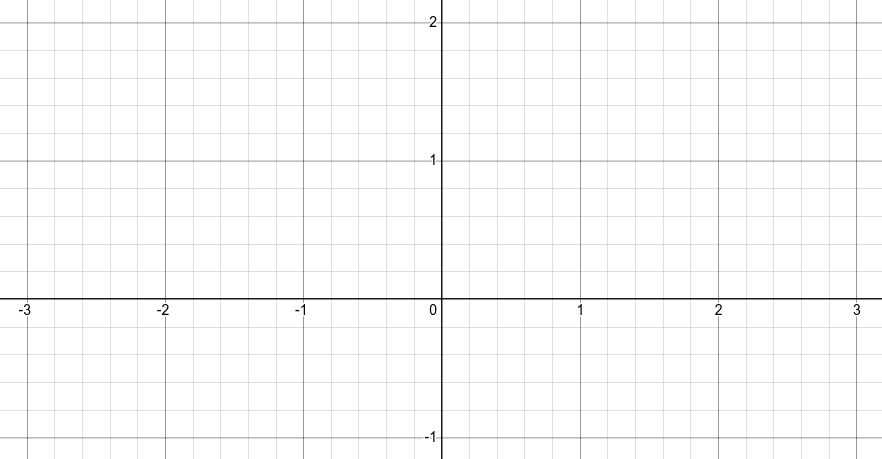
\includegraphics[scale=0.45]{GraphEmpty.png}
	\caption{Plot of $u(t)$}
	\end{figure}
	
	\subsection{Basic Operations}
	
	\begin{itemize}
	\item Translation by $a$ units:
		\begin{align*}
		u(t - a) = \left\{ 
			\begin{matrix}
			0 & t < a \\
			1 & t \geq a .
			\end{matrix} \right.
		\end{align*}
	\item Multiplication by $c$:
		\begin{align*}
		c u(t) = \left\{
			\begin{matrix}
			0 & t < 0 \\
			c & t \geq 0 .
			\end{matrix} \right.
		\end{align*}
	\item Activation of a function $f(t)$ at time $a$:
		\begin{align*}
		f(t) u (t - a) = \left\{
			\begin{matrix}
			0 & t < a \\
			f(t) & t \geq a .
			\end{matrix}
			\right.
		\end{align*}
	\item Destruction of a function $f(t)$ at time $b$ and activation of a function $g(t)$ at time $b$:
		\begin{align*}
		f(t) u(t - a) + (g(t) - f(t)) u(t - b) = \left\{
			\begin{matrix}
			0 & t < a \\
			f(t) & a \leq t < b \\
			g(t) & b \leq t .
			\end{matrix} \right.
		\end{align*}
	\end{itemize}
	
	\newpage
	
	\begin{example}
	Rewrite the function $f(t)$ in Example \ref{Exa:PieceWiseFct} using the unit step function.
	\end{example}
	
	
	\newpage
	
	\begin{example}
	A farmer has a field of potatoes of $1$ kilometer long. An automated watering system starts at 5:00\textsc{AM} and stops at 8:00\textsc{AM}. The spite of water is 1000 liters per hour. Give an expression of the function $W(t)$ of water used during the day using the unit step function.
	\end{example}
	
	
	\newpage
	
	\section{Laplace Transform of The Unit Step Function}
	Let $a \geq 0$ be a real number and $f$ be a function with a Laplace transform $F(s)$.
		\begin{itemize}
		\item $L (u (t - a)) = \displaystyle \frac{e^{-s a}}{s}$.
		\item $L (u (t- a) f(t)) = \displaystyle e^{-sa} L(f(t + a))$.
		\item $L (u(t-a) f(t-a)) = \displaystyle e^{-sa} F(s)$.
		\end{itemize}
		
	\vspace*{16pt}
	
	\begin{example}
	Find the Laplace transform of
		\begin{align*}
		f(t) = \left\{
			\begin{matrix}
			\sin (t) & , 0 \leq t < \pi / 2 \\
			\cos (t) - 3 \sin (t) & , \pi/2 \leq t < \pi \\
			3 \cos (t) & , t \geq \pi .
			\end{matrix} \right.
		\end{align*}
	\end{example}
	
	\newpage
	
	%\phantom{2}
	
	%\newpage
	
	\begin{example}
	Find
		\begin{align*}
		L^{-1} \Big( \frac{1}{s^2} - e^{-s} \big( \frac{1}{s^2} + \frac{2}{s} \big) + e^{-4s} \big( \frac{4}{s^3} + \frac{1}{s} \big) \Big)
		\end{align*}
	\end{example}
	
	\newpage
	
	\section{ODE Revisited}
	We can now allow the forcing function to be a discontinuous function (piecewise continuous).
	
	\begin{example}
	Solve the initial value problem
		\begin{align*}
		y'' - y = f(t) , \quad y(0) = -1 , \, y' (0) = 2 ,
		\end{align*}
	where
		\begin{align*}
		f(t) = \left\{ 
			\begin{matrix}
			t & 0 \leq t < 1 \\
			1 & t \geq 1 .
			\end{matrix} \right.
		\end{align*}
	\end{example}
	
	\newpage
	
	\phantom{2}
	
	\newpage
	
	\phantom{2}

\end{document}